\documentclass[cameraready]{Interspeech}

\usepackage[T1]{fontenc}
\usepackage[french]{babel}
\usepackage{graphicx}
\usepackage{booktabs}

\title{Extraction automatique de réseaux de personnages dans le cycle de Fondation}

\author[affiliation={1}]{Idir}{Namane}
\author[affiliation={1}]{Mokrane}{Slimani}
\address{$^1$CERI, Avignon Université, France}
\email{idir.namane@alumni.univ-avignon.fr}

\keywords{réseaux de personnages, reconnaissance d'entités nommées, résolution d'alias, co-occurrences}

\begin{document}

\maketitle

\begin{abstract}
Nous présentons un pipeline séquentiel qui extrait un réseau de personnages par chapitre de romans d'Asimov :
reconnaissance d'entités nommées avec spaCy étendue aux titres, filtrage de faux personnages par des indices
appris sur le corpus, rappel des noms validés dans tout le livre, résolution d'alias et de surnoms au niveau du
livre, puis graphe de co-occurrences à 25 tokens. Sur le leaderboard Kaggle du défi, le score passe de 0,482
pour une baseline à 0,741. Une métrique recodée et quatre passages annotés de la trilogie Fondation donnent une
évaluation locale (0,900) et une analyse des erreurs. Les réseaux par livre retrouvent la structure en parties
des romans ; les erreurs restantes viennent surtout des noms de famille partagés, des titres et des identités
cachées.
\end{abstract}

\section{Introduction}

Un réseau de personnages résume une œuvre de fiction : chaque nœud est un personnage, chaque arête une
interaction~\cite{labatut2019}. L'extraire automatiquement demande d'enchaîner plusieurs tâches de TALN : détecter
les mentions de personnages (reconnaissance d'entités nommées, REN), regrouper les mentions d'un même personnage
(résolution d'alias~\cite{vala2015}), détecter les interactions, ici approchées par les co-occurrences, puis
construire le graphe. Chaque étape propage ses erreurs aux suivantes : un lieu pris pour un personnage ajoute un
nœud et des arêtes fausses, un alias mal rattaché coupe un personnage en deux.

Le défi porte sur des romans du cycle de Fondation d'Isaac Asimov, en français. Il faut produire un graphe par
chapitre de \emph{Prélude à Fondation} et des \emph{Cavernes d'acier} (37 chapitres, 118\,000 mots) pour un
leaderboard Kaggle, et un réseau par livre de la trilogie \emph{Fondation}, \emph{Fondation et Empire},
\emph{Seconde Fondation}, à commenter qualitativement. Nous avons choisi un pipeline à base de règles, autour
d'un modèle de REN générique, dont chaque règle s'appuie sur des statistiques calculées sur le texte traité
plutôt que sur des listes de noms écrites à la main. Le code est
public\footnote{\url{https://github.com/idirnamane27-blip/Reseaux-personnages-fondation}}.

\section{Tâche et évaluation}

Deux mentions sont en co-occurrence quand elles sont séparées par 25 tokens ou moins ; le poids d'une arête est
le nombre de co-occurrences. Chaque nœud porte l'attribut \texttt{names}, la liste de ses alias. D'après les
consignes d'annotation, les titres font partie de l'entité («~Dr Sarton~»), un nom commun à majuscule qui désigne
une personne précise est annoté avec son article («~le Maire~»), et les gentilés («~les Spaciens~») ne le sont pas.

Le score est la moyenne de deux F1. Pour les nœuds, la précision suit~\cite{vala2015} : couplage biparti maximal
avec $sim_p(E,G)=1-|E-G|/|E|$, qui pénalise chaque nom prédit en trop ; le rappel compte les personnages de
référence qui partagent au moins un nom avec leur nœud couplé. Pour les arêtes, les nœuds sont couplés par
l'indice de Jaccard de leurs noms, et une arête prédite est juste si ses deux extrémités sont couplées à deux
nœuds reliés dans la référence. Comme les noms sont comparés à l'identique, un nœud «~Dorwin~» ne correspond pas
à la référence «~seigneur Dorwin~» : il compte à la fois comme un nœud en trop et comme un personnage manqué.

\textbf{Évaluation locale.} Les soumissions Kaggle sont limitées et ne disent pas quelles erreurs coûtent des
points. Nous avons recodé la métrique (couplage par l'algorithme hongrois de SciPy) et annoté quatre passages de
5 pages de la trilogie (environ 1\,600 mots chacun) : le début de \emph{Fondation} (2 personnages), la crise du
caveau de Hardin (8), Magnifico et Indbur dans \emph{Fondation et Empire} (9), le Mulet face au Premier Orateur
dans \emph{Seconde Fondation} (5). Les références listent les formes de chaque personnage ; leurs occurrences et
leurs liens sont retrouvés automatiquement avec la même règle des 25 tokens. Le sujet demande de ne pas annoter
les chapitres du leaderboard : ces passages mesurent donc aussi la généralisation à d'autres livres.

\section{Pipeline}

\textbf{REN.} Nous gardons les entités \texttt{PER} du modèle \texttt{fr\_core\_news\_md} de
spaCy~\cite{spacy}, étendues au titre qui les précède («~docteur Seldon~», «~R.~Daneel~») d'après une liste de
titres. Le texte est d'abord remis sur une ligne, en recollant les traits d'union de fin de ligne, et la
signature des citations de l'\emph{Encyclopaedia Galactica} est retirée : spaCy la collait au nom qui suit.

\textbf{Filtre.} spaCy prend pour des personnes des mots de début de réplique («~Vraiment~»), des lieux
(«~Trantor~») et des gentilés. Pour un nom d'un seul mot, les indices sont appris sur le corpus traité, dans
cet ordre : (1) suffixe de gentilé (\mbox{-ien}, \mbox{-ite}) ; (2) un mot sujet d'au moins deux incises
(«~fit Mis~», «~dit le Mulet~») est une personne sûre, les verbes de parole étant appris sur les formes
«~dit-il~», «~demanda-t-elle~» ; (3) un mot plus souvent écrit en minuscule qu'avec une majuscule en milieu de
phrase est rejeté ; (4) un lieu suit souvent «~sur, vers, dans, depuis~» (10\,\%), «~à~» (15\,\%), «~de~»
(50\,\%) ou un article (50\,\%) ; (5) un nom commun du lexique Lexique~\cite{lexique} employé seul
(«~Excellence~») est rejeté, mais un titre prouve la personne («~R.~Sammy~»). Sur le leaderboard, le filtre
retire 419 des 2\,159 mentions de spaCy : 257 lieux (Trantor 94, Mycogène 56, Dahl 26), 66 mots de début de
réplique, 52 noms communs (dont Kan, un secteur de Trantor) et 42 gentilés. Nous n'utilisons pas le vote LOC
contre PER de spaCy : il étiquette «~Seldon~» comme lieu plus souvent que comme personne. Les bords d'entité mal
placés sont corrigés («~Jéhu galopa~», «~Mulet - conquérant~», et «~Grimace de Seldon~» en début de phrase).
Enfin, l'article fait partie du nom quand le nom le suit souvent («~le Mulet~», «~le Premier Orateur~»).

\textbf{Rappel.} Un nom validé une fois dans un livre est recherché dans tous ses chapitres, avec le même
découpage en tokens que spaCy ; en cas de chevauchement, la mention la plus longue gagne. Sur le leaderboard, le
nombre de mentions passe de 1\,740 à 2\,956.

\textbf{Résolution d'alias.} Elle est faite sur le livre entier, puis restreinte à chaque chapitre : «~Lije~»
rejoint Baley même dans un chapitre où «~Lije Baley~» n'apparaît pas. Sans les titres ni la casse, un nom long
absorbe ceux qu'il contient ; un nom d'un mot rejoint le nom long le plus cité qui le contient (à égalité, l'ordre
alphabétique rend le résultat reproductible) ; un titre seul («~Empereur~») rejoint le seul personnage qui le
porte, sinon il est retiré. Deux règles traitent les surnoms : même nom de famille et prénoms proches
(«~Lije Baley~» et «~Elijah Baley~», mais pas «~Jessie Baley~» et «~Bentley Baley~») ; abréviation d'un nom
propre de mêmes deux premières lettres («~Ben~» et «~Bentley~», mais pas «~Mis~» et «~Ministre~»).

\section{Résultats}

Le tableau~\ref{tab:kaggle} donne l'apport de chaque étape sur le leaderboard. Le filtre (+15 points) et le
rappel (+6) apportent le plus ; les surnoms ajoutent 3 points, surtout parce que «~Lije~» formait un nœud en
double avec Baley dans 14 chapitres des \emph{Cavernes d'acier}.

\begin{table}[t]
  \caption{Score Kaggle (moyenne des F1 nœuds et arêtes) et score local sur les quatre passages annotés.}
  \label{tab:kaggle}
  \centering
  \begin{tabular}{@{}llcc@{}}
    \toprule
    & \textbf{Ajout} & \textbf{Kaggle} & \textbf{Local} \\
    \midrule
    v1 & spaCy + titres + alias par inclusion & 0,482 & \\
    v2 & filtre, bords d'entité, casse & 0,634 & \\
    v3 & rappel, alias au niveau du livre & 0,695 & \\
    v4 & surnoms & 0,726 & 0,658 \\
    v5 & locuteurs, article, noms communs & \textbf{0,741} & 0,900 \\
    v6 & rejet «~jamais en milieu de phrase~» & 0,727 & 0,966 \\
    \bottomrule
  \end{tabular}
\end{table}

Le tableau~\ref{tab:local} détaille l'évaluation locale de la v5, avec et sans rappel. Le rappel retrouve
quelques personnages ratés par spaCy, mais surtout des liens : sans lui, le rappel des arêtes tombe de 1,00 à
0,24. spaCy ne reconnaît en effet qu'une partie des occurrences d'un nom : sur le passage de \emph{Fondation et
Empire}, il trouve Magnifico une fois sur 7, Seldon une fois sur 6, Mis une fois sur 7, et jamais Toran.

\begin{table}[t]
  \caption{Évaluation locale de la v5 : F1 des nœuds (N), des arêtes (A) et score, avec et sans rappel.}
  \label{tab:local}
  \centering
  \begin{tabular}{@{}lcccccc@{}}
    \toprule
    & \multicolumn{3}{c}{\textbf{avec rappel}} & \multicolumn{3}{c}{\textbf{sans rappel}} \\
    \cmidrule(lr){2-4}\cmidrule(l){5-7}
    \textbf{Passage} & N & A & score & N & A & score \\
    \midrule
    Fondation, début & 0,80 & 0,67 & 0,733 & 0,80 & 0,00 & 0,400 \\
    Fondation, caveau & 0,93 & 1,00 & 0,967 & 0,93 & 0,75 & 0,842 \\
    Fondation et Empire & 0,95 & 0,98 & 0,961 & 0,88 & 0,18 & 0,528 \\
    Seconde Fondation & 0,88 & 1,00 & 0,938 & 0,80 & 0,40 & 0,600 \\
    \midrule
    Moyenne & 0,89 & 0,91 & \textbf{0,900} & 0,85 & 0,33 & 0,593 \\
    \bottomrule
  \end{tabular}
\end{table}

Entre v4 et v5, l'évaluation locale a révélé des erreurs invisibles sur Kaggle : le Mulet pris pour un lieu, car
presque toujours précédé d'un article ; «~Ebling Mis~» rejeté, car «~mis~» existe en minuscule ; «~Premier
Orateur~» réduit à «~Orateur~». Le score local de v5 est optimiste, puisque ces règles ont été corrigées en
regardant les mêmes passages ; le gain sur Kaggle montre qu'elles se généralisent. La v6 rejette les mots jamais
vus avec une majuscule en milieu de phrase («~Atterrissez~», «~Hum~») : sur le leaderboard, elle ne retire que
17 nœuds de ce type et leurs 27 arêtes, mais le score baisse. Retirer un faux nœud ne peut qu'augmenter la
précision : soit certains de ces mots sont annotés comme personnages, soit, comme l'évaluation porte sur des
chapitres tirés au hasard, une partie de l'écart vient de l'échantillon. Nous gardons la v5.

\section{Réseaux par livre}

La trilogie (pages impaires seulement : la moitié du texte manque) est coupée en blocs de 5 pages, les alias sont
résolus par livre et les co-occurrences additionnées. Les communautés sont obtenues par optimisation gloutonne de
la modularité~\cite{clauset2004}, l'intermédiarité avec la distance $1/\textrm{poids}$~\cite{brandes2001}. Le
tableau~\ref{tab:livres} résume les trois réseaux et les figures~\ref{fig:fee}, \ref{fig:sdf} et~\ref{fig:fon} montrent leur
composante principale.

\begin{table}[t]
  \caption{Réseaux par livre : personnages, liens, densité et personnage le plus central (degré).}
  \label{tab:livres}
  \centering
  \begin{tabular}{@{}lcccl@{}}
    \toprule
    \textbf{Roman} & \textbf{Pers.} & \textbf{Liens} & \textbf{Densité} & \textbf{Central} \\
    \midrule
    Fondation & 64 & 101 & 0,050 & Salvor Hardin (26) \\
    Fondation et Empire & 47 & 111 & 0,103 & le Mulet (20) \\
    Seconde Fondation & 49 & 87 & 0,074 & docteur Darell (12) \\
    \bottomrule
  \end{tabular}
\end{table}

\begin{figure*}[t]
  \centering
  \begin{minipage}[t]{0.49\textwidth}
    \centering
    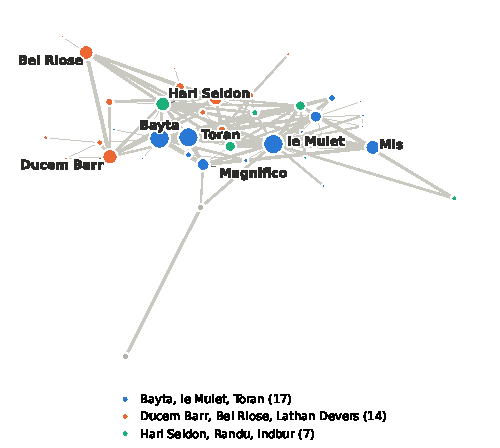
\includegraphics[width=\linewidth]{figures/fee.pdf}
    \caption{\emph{Fondation et Empire} : les deux parties du roman (le Mulet, en bleu ; le général Riose, en
    orange), reliées par Hari Seldon.}
    \label{fig:fee}
  \end{minipage}\hfill
  \begin{minipage}[t]{0.49\textwidth}
    \centering
    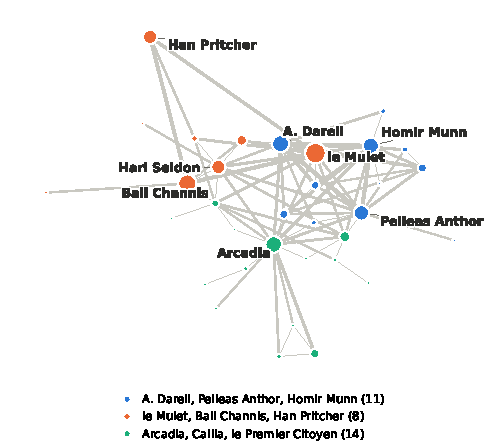
\includegraphics[width=\linewidth]{figures/sdf.pdf}
    \caption{\emph{Seconde Fondation} : la quête du Mulet (orange), les conspirateurs de Terminus (bleu) et le
    voyage d'Arcadia (vert). «~A.~Darell~» désigne en fait le docteur Darell (voir section~\ref{sec:erreurs}).}
    \label{fig:sdf}
  \end{minipage}
\end{figure*}

\begin{figure}[t]
  \centering
  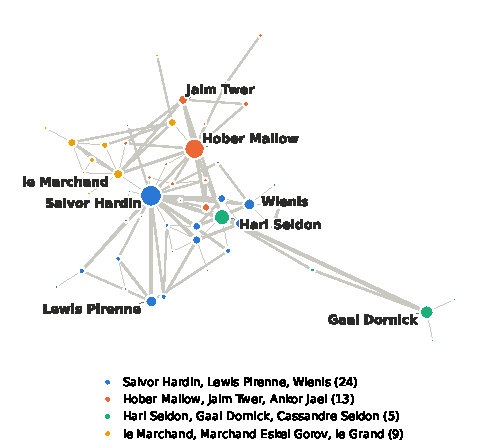
\includegraphics[width=\columnwidth]{figures/fon.pdf}
  \caption{\emph{Fondation} : une communauté par épisode (Hardin en bleu, Mallow en orange, Seldon et Gaal
  Dornick en vert, les Marchands en jaune). Taille du nœud : mentions ; épaisseur : co-occurrences.}
  \label{fig:fon}
\end{figure}

Dans les trois romans, les communautés retrouvent les parties de l'intrigue. \emph{Fondation} est un recueil de
nouvelles séparées par des décennies ; c'est le réseau le moins dense, et ses communautés correspondent aux
épisodes (figure~\ref{fig:fon}). Les deux nouvelles dont Salvor Hardin est le héros n'en forment qu'une, puisque
le même personnage les relie ; Hardin a la plus forte intermédiarité (0,49). Dans \emph{Fondation et Empire}
(figure~\ref{fig:fee}), le réseau est le plus dense, car la seconde partie suit quatre personnages qui voyagent
ensemble (Bayta, Toran, Magnifico, Mis). Le Mulet est le personnage le plus central alors qu'il n'apparaît
presque pas en personne avant la fin : on parle de lui sans cesse, ce qui montre qu'une co-occurrence n'est pas
une interaction. Dans \emph{Seconde Fondation} (figure~\ref{fig:sdf}), les trois communautés suivent les trois
fils de l'intrigue. Enfin, Hari Seldon relie les époques dans les trois réseaux (intermédiarité 0,36 dans
\emph{Fondation}, 0,27 dans \emph{Fondation et Empire}) alors qu'il meurt dans la première partie du cycle : ses
apparitions enregistrées et les références à son Plan en font le fil conducteur de la série.

\section{Analyse des erreurs}
\label{sec:erreurs}

\textbf{Identités cachées.} Magnifico, le bouffon, \emph{est} le Mulet, ce que le lecteur n'apprend qu'à la
fin : ils forment deux nœuds reliés par 7 co-occurrences. De même pour Preem Palver et le Premier Orateur. Aucune
méthode fondée sur les noms ne peut les réunir ; pour un lecteur qui découvre le livre, le graphe est d'ailleurs
fidèle.

\textbf{Noms et titres partagés.} «~Darell~» seul est rattaché au nom long le plus cité qui le contient,
«~A.~Darell~» (une signature d'Arcadia), alors qu'il désigne surtout son père ; Arcadia forme son propre nœud, et
ses ancêtres Bayta et Toran Darell, cités, sont isolés. Un nom de famille porté par toute une famille ne peut pas
être résolu par inclusion de noms. De même, «~Premier Citoyen~» est le titre du Mulet dans la première partie et
de Stettin dans la seconde : les deux sont fusionnés, ce qui relie à tort les deux époques. Une résolution d'alias
limitée à une fenêtre de chapitres, ou guidée par les co-occurrences, éviterait une partie de ces fusions.

\textbf{Rappel des noms seuls.} Limmar Ponyets, héros d'une nouvelle de \emph{Fondation}, n'a qu'une mention :
«~Ponyets~» seul n'est jamais reconnu par spaCy, et le rappel ne cherche que les noms déjà validés. Chercher aussi
le nom de famille seul des noms complets validés corrigerait ce cas, au risque de nouvelles confusions (Darell).
En local, «~Alurin~», cité une seule fois dans tout le livre et non reconnu par spaCy, ne peut être retrouvé par
aucune étape.

\textbf{Formules d'adresse et mots isolés.} «~Majesté Impériale~» (Cléon II) et «~le Marchand~» (Devers) restent
séparés de leur porteur, faute de nom propre à côté. Des impératifs («~Calmez~»), des onomatopées («~Hmmm~») et
des expressions («~talon d'Achille~») subsistent quand ils ne sont jamais écrits en minuscule ailleurs.

\section{Conclusion}

Un pipeline à base de règles apprises sur le corpus, autour d'une REN générique, atteint 0,741 sur le leaderboard,
contre 0,482 pour la baseline. L'étape la plus utile est le rappel des noms validés dans le livre, qui retrouve
surtout des liens. L'évaluation locale sur des passages annotés a permis de trouver des erreurs qu'un score global
ne montre pas, et de vérifier que les règles se généralisent à d'autres livres. Les erreurs restantes relèvent
de la résolution d'alias plus que de la REN. Les pistes suivantes sont la résolution de coréférence, qui
rattacherait les pronoms et les descriptions («~le bouffon~») aux personnages, des réseaux dynamiques par partie
de roman, et un modèle de REN affiné sur des textes littéraires.

\bibliographystyle{IEEEtran}
\bibliography{mybib}

\end{document}
